\documentclass{article}
\usepackage[utf8]{inputenc}
\usepackage[]{amsmath, graphicx}
\usepackage[dvipsnames]{xcolor}

\usepackage[backend=biber,style=alphabetic,sorting=ynt]{biblatex}
\addbibresource{phstr.bib}

\title{Put a title: LMG}
\author{M Rahaman, A Roy, T Mori}
\begin{document}
\maketitle

\section{Introduction}
Dynamical Freezing (DMF) is a phenomenon whereby periodically driven Many Body Systems are prevented from thermalizing to infinite temperature due to a dynamical hysteresis that prevents observables from reaching their diagonal averaged values.

DMF can, under certain resonance conditions in the drive parameters, cause the response to ‘freeze’ completely to its initial value for all times\cite{ArnabD}. This has been demonstrated (via the Jordan-Wigner Transformation) in the driven TFIM with nearest neighbour interactions and is shown to be protected when translational invariance is explicitly broken (say, by disorder). 

We have suspected that this is also protected against the loss of other symmetries, for example, in long range systems where JW transformation produces nonlocalities. To prove this, we introduce a long-range power-law dependence in the TFIM, where the exchange $J_{ij}\sim 1/|i-j|^\beta$. Here, for $\beta=\infty$, we recover the short range TFIM and freezing at resonant drive parameters. When $\beta=0$, taking $N\rightarrow\infty$ allows us to describe the exact dynamics by the periodically driven Lipkin-Meshkov-Glick (LMG) model, which we have solved numerically to obtain a similar kind of DMF and ‘freezing’ as the$\beta=\infty$ case.

Now, we compare the degree of localization of the quasi-stationary Floquet modes in both cases. In order to do so, we look at the Inverse Participation Ratios (IPR) of the modes in the representation given by the eigenstates of the symmetry-breaking field. 

What we're seeing is that there appears to be a high degree of localization in the TFIM case, as consistent with analytical treatments using the Rotated Wave Approximation (RWA), where only the slowest rotating terms in the Fourier expansion of the Hamiltonian in a frame co-rotating with the symmetry-breaking driving field are retained. However, this localization remains qualitatively strong even at lower drive frequencies where RWA breaks down.

In the driven LMG model, the localization is similar to the Ising model for high frequencies but breaks down substantively at lower frequencies due to the onset of dynamical chaos in the thermodynamic limit. Thus, a change of phase should occur from a thermal state to an athermal one if the drive frequency is varied adiabatically.

\subsection{Background}
A generic interacting quantum many body system, if driven time-periodically for a sufficiently long time, is expected to follow a dynamical route to thermalization at infinite temperature. This can be demonstrated by the Eigenstate Thermalization Hypothesis (ETH), where long-time averages of observables, resolved in the basis of stationary states, approach the average predicted by the microcanonical ensemble. 

For instance, if the stationary states are expressed by $|e_i\rangle$, with corresponding eigenvalues $e_i$ of Hamiltonian $H$, then the time-evolution of an observable $O$ on a closed isolated quantum system starting from $|\psi_0\rangle$ at $t=0$ is
\begin{align*}
\langle O (t) \rangle &= \langle e^{iHt}Oe^{-iHt}\rangle\\
                      &= \sum_{ij}e^{-i\big(e_i-e_j\big)t} O_{ij} \langle\psi_0|e_i\rangle \langle e_j|\psi_0\rangle.
\end{align*}
The time-average of this expectation, averaged over very long times and non-degenerate $e_i$, is expected to be
\begin{align*}
\overline{\langle O (t) \rangle} &= \sum_{ij}\overline{e^{-i\big(e_i-e_j\big)t}}O_{ij} \langle\psi_0|e_i\rangle \langle e_j|\psi_0\rangle\\
 &= \sum_{ij}\delta_{ij}O_{ij} \langle\psi_0|e_i\rangle \langle e_j|\psi_0\rangle\\
 &=\sum_i O_{ii}\bigg\vert \langle e_i\vert\psi_0\rangle \bigg\vert^2,
\end{align*}
Thus, after a long time, $\overline{O}$ reaches a diagonal average that, under the conditions of ETH, should thermalize. However, a high degree of degeneracy in the eigenvalues $e_i$ will prevent some of the $\overline{e^{-i\big(e_i-e_j\big)t}}$-terms from reaching $\delta_{ij}$. In the extreme case when all the eigenvalues are equal, the diagonal average values are dynamically suppressed, leading to Dynamical Many Body Localization or Many Body Freezing. We want to look at the localization of Floquet eigenstates in this regime.


\subsection{Investigation of IPR in the Floquet Dynamics of Many Body Systems}
We're trying to look at localization/freezing in rapidly driven time-periodic systems. Specifically, we want to check whether freezing exists in long raange spin systems in the manner seen for short range systems. We start by defining the *Inverse Participation Ratio* (IPR) for a wavefunction $\psi(x)$ as 
\begin{equation*}
\phi_{IPR}\equiv \int dx\;\vert\psi(x)\vert^4
\end{equation*}

More generally, the IPR of a state $|\phi\rangle$ in a representation given by complete orthonormal basis $|m\rangle$ is $\phi_{IPR} = \sum_m\vert\langle m \vert\phi\rangle\vert^4$.

In the context of localization, the IPR is useful. The smallest value of the IPR corresponds to a fully delocalized state, $\psi(x)=1/\sqrt{N}$ for a system of size $N$, where the IPR yields $\sum_x |\psi(x)|^4=N/(N^{1/2})^4=1/N$. Values of the IPR close to 1 correspond to localized states. For a periodically driven system, we look at the IPR of the Floquet modes at $t=T$, where $t=2\pi/\omega$ for drive frequency $\omega$.


\section{Transverse-Field Ising model}
First, consider the well-known Hamiltonian of the driven Transverse Field Ising model of $N$ spins:
\begin{align*}
 H(t) &= H_0 + \left(h_0 + h\cos{\omega t}\right) H_1\\
H_0 &= -\frac{1}{2}\sum_{i} \sigma^x_i \sigma^x_{i+1}\\
H_1 &= -\frac{1}{2}\sum_n^N \sigma^z_{n}
\end{align*}

The TFIM model can be readily transformed into a Bogoliubov-type fermionic system via the Jordan-Wigner transformation. This yields an effective Hamiltonian

\begin{equation*}
\mathcal{H}(t)=\sum_{{k, -k}} \psi_{{k}}^{\dagger}\left(\begin{array}{cc}
h_{z}(t)+f_{{k}} & \Delta_{{k}} \\
\Delta_{{k}}^{*} & -h_{z}(t)-f_{{k}}
\end{array}\right) \psi_{{k}},
\end{equation*}

where $h_z(t) = h_0 + h\cos{\omega t}$, $\psi_k = (c_{-k}, c^\dagger_k)^T$, with $f_k = J\cos{k}$, $\Delta_k = J\sin{k}$. We can rewrite

\begin{equation*}
H(t) = \sum_{k,-k} \psi^\dagger_k
\Big[\sigma_z f_k + \sigma_x \Delta_k + \sigma_z h_z(t)\Big]\psi_k
\end{equation*}

For a particular $k,-k$ pair, let us define the undriven part $H_0(k) = \sigma_z f_k + \sigma_x \Delta_k$ and $H_1 = \sigma_z$, yielding 
$H_k(t) = H_0(k) + h\cos{\omega t}\; H_1$. Now, we transform to the rotated frame via the unitary transformation operator $U = e^{i\int H_d d t} = exp \Big[\frac{i h}{\omega}\sin{\omega t}\Big]\sigma_z$. This yields
\begin{align*}
H^\prime_k(t) &= U^\dagger H_0(k) U \\
&=e^{-i\frac{h}{\omega}\sin{\omega t}\sigma_z} H_0(k) e^{i\frac{h}{\omega}\sin{\omega t}\sigma_z}\\
\end{align*}


If we define defined $\eta=2h/\omega$, then
\begin{align*}
H^\prime_k(t) &= \begin{pmatrix}e^{-i\frac12\eta\sin{\omega t}}&0\\0&e^{i\frac12\eta\sin{\omega t}}\end{pmatrix} \begin{pmatrix}f_k&\Delta_k\\\Delta_k &-f_k\end{pmatrix}\begin{pmatrix}e^{i\frac12\eta\sin{\omega t}}&0\\0&e^{-i\frac12\eta\sin{\omega t}}\end{pmatrix}\\
&= \begin{pmatrix}f_k&e^{i\eta\sin{\omega t}}\Delta_k\\e^{-i\eta\sin{\omega t}}\Delta_k&-f_k\end{pmatrix}\\
&=  \sigma^z f_k + 2\sigma^x \Delta_k \sum_{n\geq 0} J_{2n}(\eta)\cos{\big(2n\omega t\big)} - 2\sigma^y\Delta_k \sum_{n\geq 0} J_{2n+1}(\eta)\sin{\bigg[\big(2n+1\big)\omega t\bigg]}
\end{align*}
Here, in the last step, have used the Jacobi-Anger formula $e^{i \eta \sin{\omega t}} \equiv \sum_{n=-\infty}^{\infty} J_n(\eta)\, e^{i n \omega t}$ \cite{Miao}. Now, for large $\omega \gg f_k$, the RWA approximation allows us to replace $H^\prime_k(t)$ by its long-time average, leaving behind only the non-oscillating modes in the expansion above, an effective Hamiltonian [1]
\begin{equation*}
H^{(RWA)}_k=f_k \sigma^z + 2 J_0(\eta)\Delta_k\sigma^x.
\end{equation*}
Clearly, if we adjust drive parameters such that $\eta$ lies on a root of $J_0(\eta)$, then $\sigma^z$ becomes a conserved quantity. A particular Floquet mode of the Hamiltonian can, in general, be written as $|\phi\rangle = \prod_{k,-k}|\phi^n_k\rangle$. In the RWA limit and in the regime where $J_0(\eta)$ vanishes, $|\phi^n_k\rangle$ has values of $|0\rangle, |k,-k\rangle$ for two values of $n=0,1$ respectively.

We define the reduced IPR of $|\phi^n_k\rangle\; \forall k$ to be
\begin{equation}
\label{eq:redipr:ising}
\phi^{(n)}_{IPR}(k) = \left\vert \langle 0 |\phi^n_k\rangle  \right\vert^4 + \left\vert \langle +k, -k |\phi^n_k\rangle  \right\vert^4,
\end{equation}
where $n=0,1$. In the RWA limit, when $J_0(eta)$ vanishes, this quantity is unity, indicating low participation and high degree of localization.


The code cell below plots $\phi^n_{IPR}(k)$ for the full exact dynamics, with different drive amplitudes $h$, and $\omega = 90$ fixed.


\begin{figure}[]
\centering
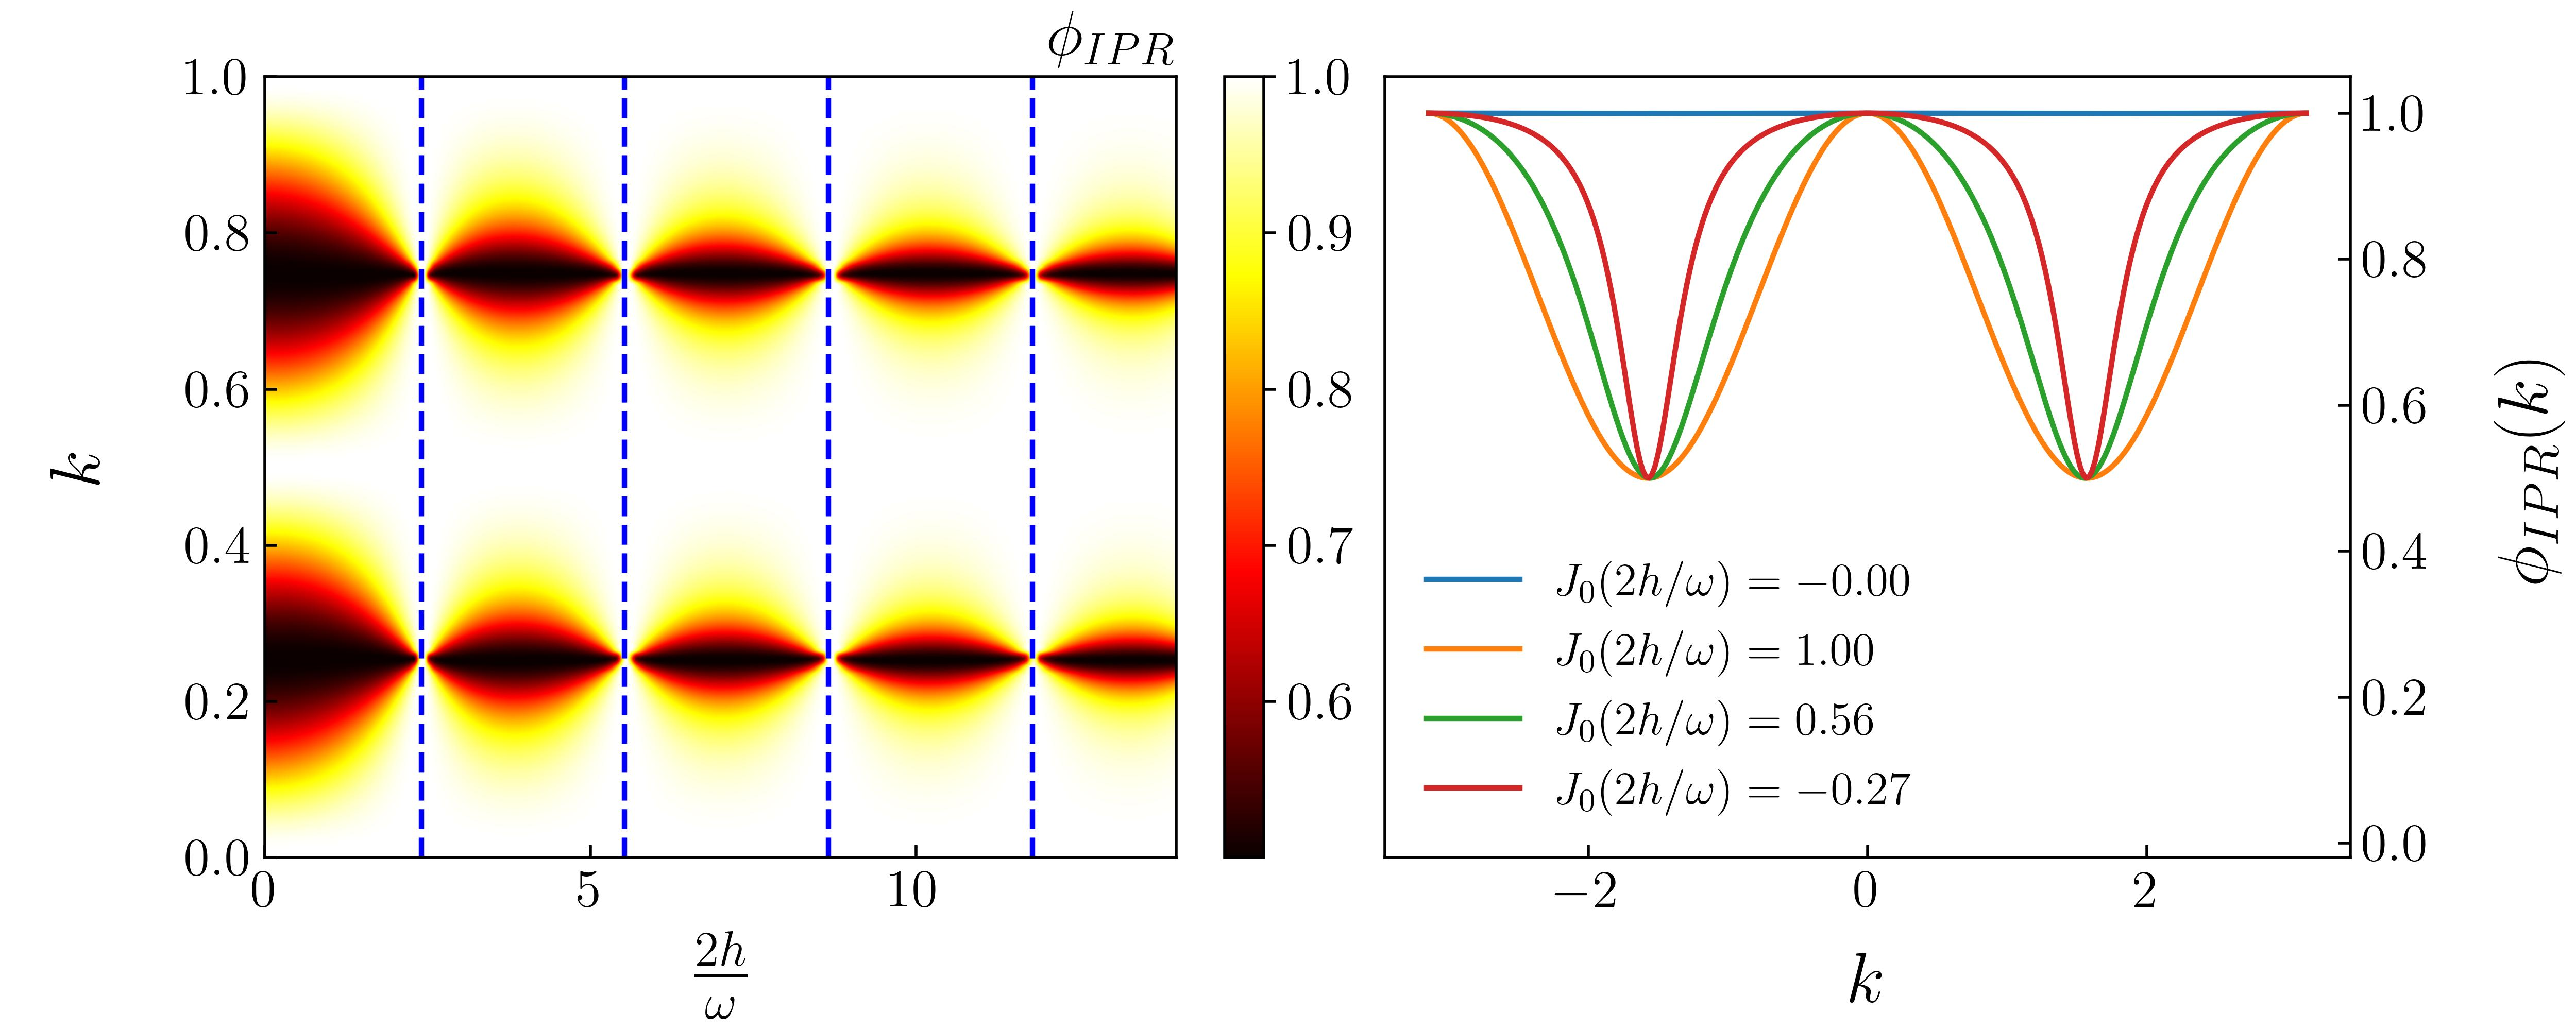
\includegraphics[height = 5cm, width = 12cm]{ising_exact_ipr.jpeg}
\caption{The plots above are for the exact dynamics of the TFIM in Fermionic representation for size N = 100, with the reduced IPR (defined in equation~\ref{eq:redipr:ising}) plotted for the entire Brillouin zone for a few drive amplitudes. The frequency is set to $\omega = 90$ and the IPR of one of the two Floquet modes are plotted at time $t=T$ for four different chosen amplitudes. The exact result is consistent with the RWA approximation. When $J_0(2h/\omega) = 0$, the RWA Hamiltonian vanishes, yielding an IPR of unity. At other points, the IPR is unity only when $k=\pm \pi$ (since $\Delta_k=0$) and $k=0$ (since $f_k = 0$ and the Hamiltonian for each $k$ $\sim \sigma_x$); other than that, there is delocalization due to the ensuing dynamics.}
\end{figure}

Finally, let us look at quantitative comparisons between the exact result and the RWA result.  We compare IPR's of the Floquet modes obtained with the zeroth and first order terms in the RWA expansion with the exact case. The three Hamiltonians whose Floquet modes are to be compared are
\begin{align*}
H_k(t) &= \sigma_z f_k + \sigma_x \Delta_k + \sigma_z h\cos{\omega t}\\
H^{(RWA)}_k(t) &= \sigma_z f_k + 2 J_0(\eta) \sigma^x \Delta_k\\
H^{(RWA2)}_k(t) &= H^{(RWA)}_k(t) - 2 J_1(\eta)\Delta_k \sigma^y\;\sin{\big(\omega t\big)}. 
\end{align*}
with $\eta=2 h/\omega$. 
\subsection{Ising model at higher symmetry breaking field frequencies}
\begin{figure}[ht!]
\centering
\includegraphics[height = 14.0cm, width = 12cm]{ising_ipr_exact_rwa_order_5_N_30.jpeg}
\caption{\color{blue}The IPR for system size N = 200 's exact dynamics and with RWA order correction are plotted here. RWA on exact Hamiltonian shows at finite size N$\sim$ 30 lattice it requires significant higher order approximation to yield replica of exact dynamics.}
\end{figure}

\subsection{Ising model at small symmetry breaking field frequencies}
We now show IPR plots of the Ising model at low drive frequency $h, \omega = \mathcal{O}(1)$ (specifically $\omega=2$). At such low frequencies, RWA breaks down, but localization persists nonetheless, as can be seen in the {\color{blue} plot} below.
\begin{figure}[ht!]
\centering
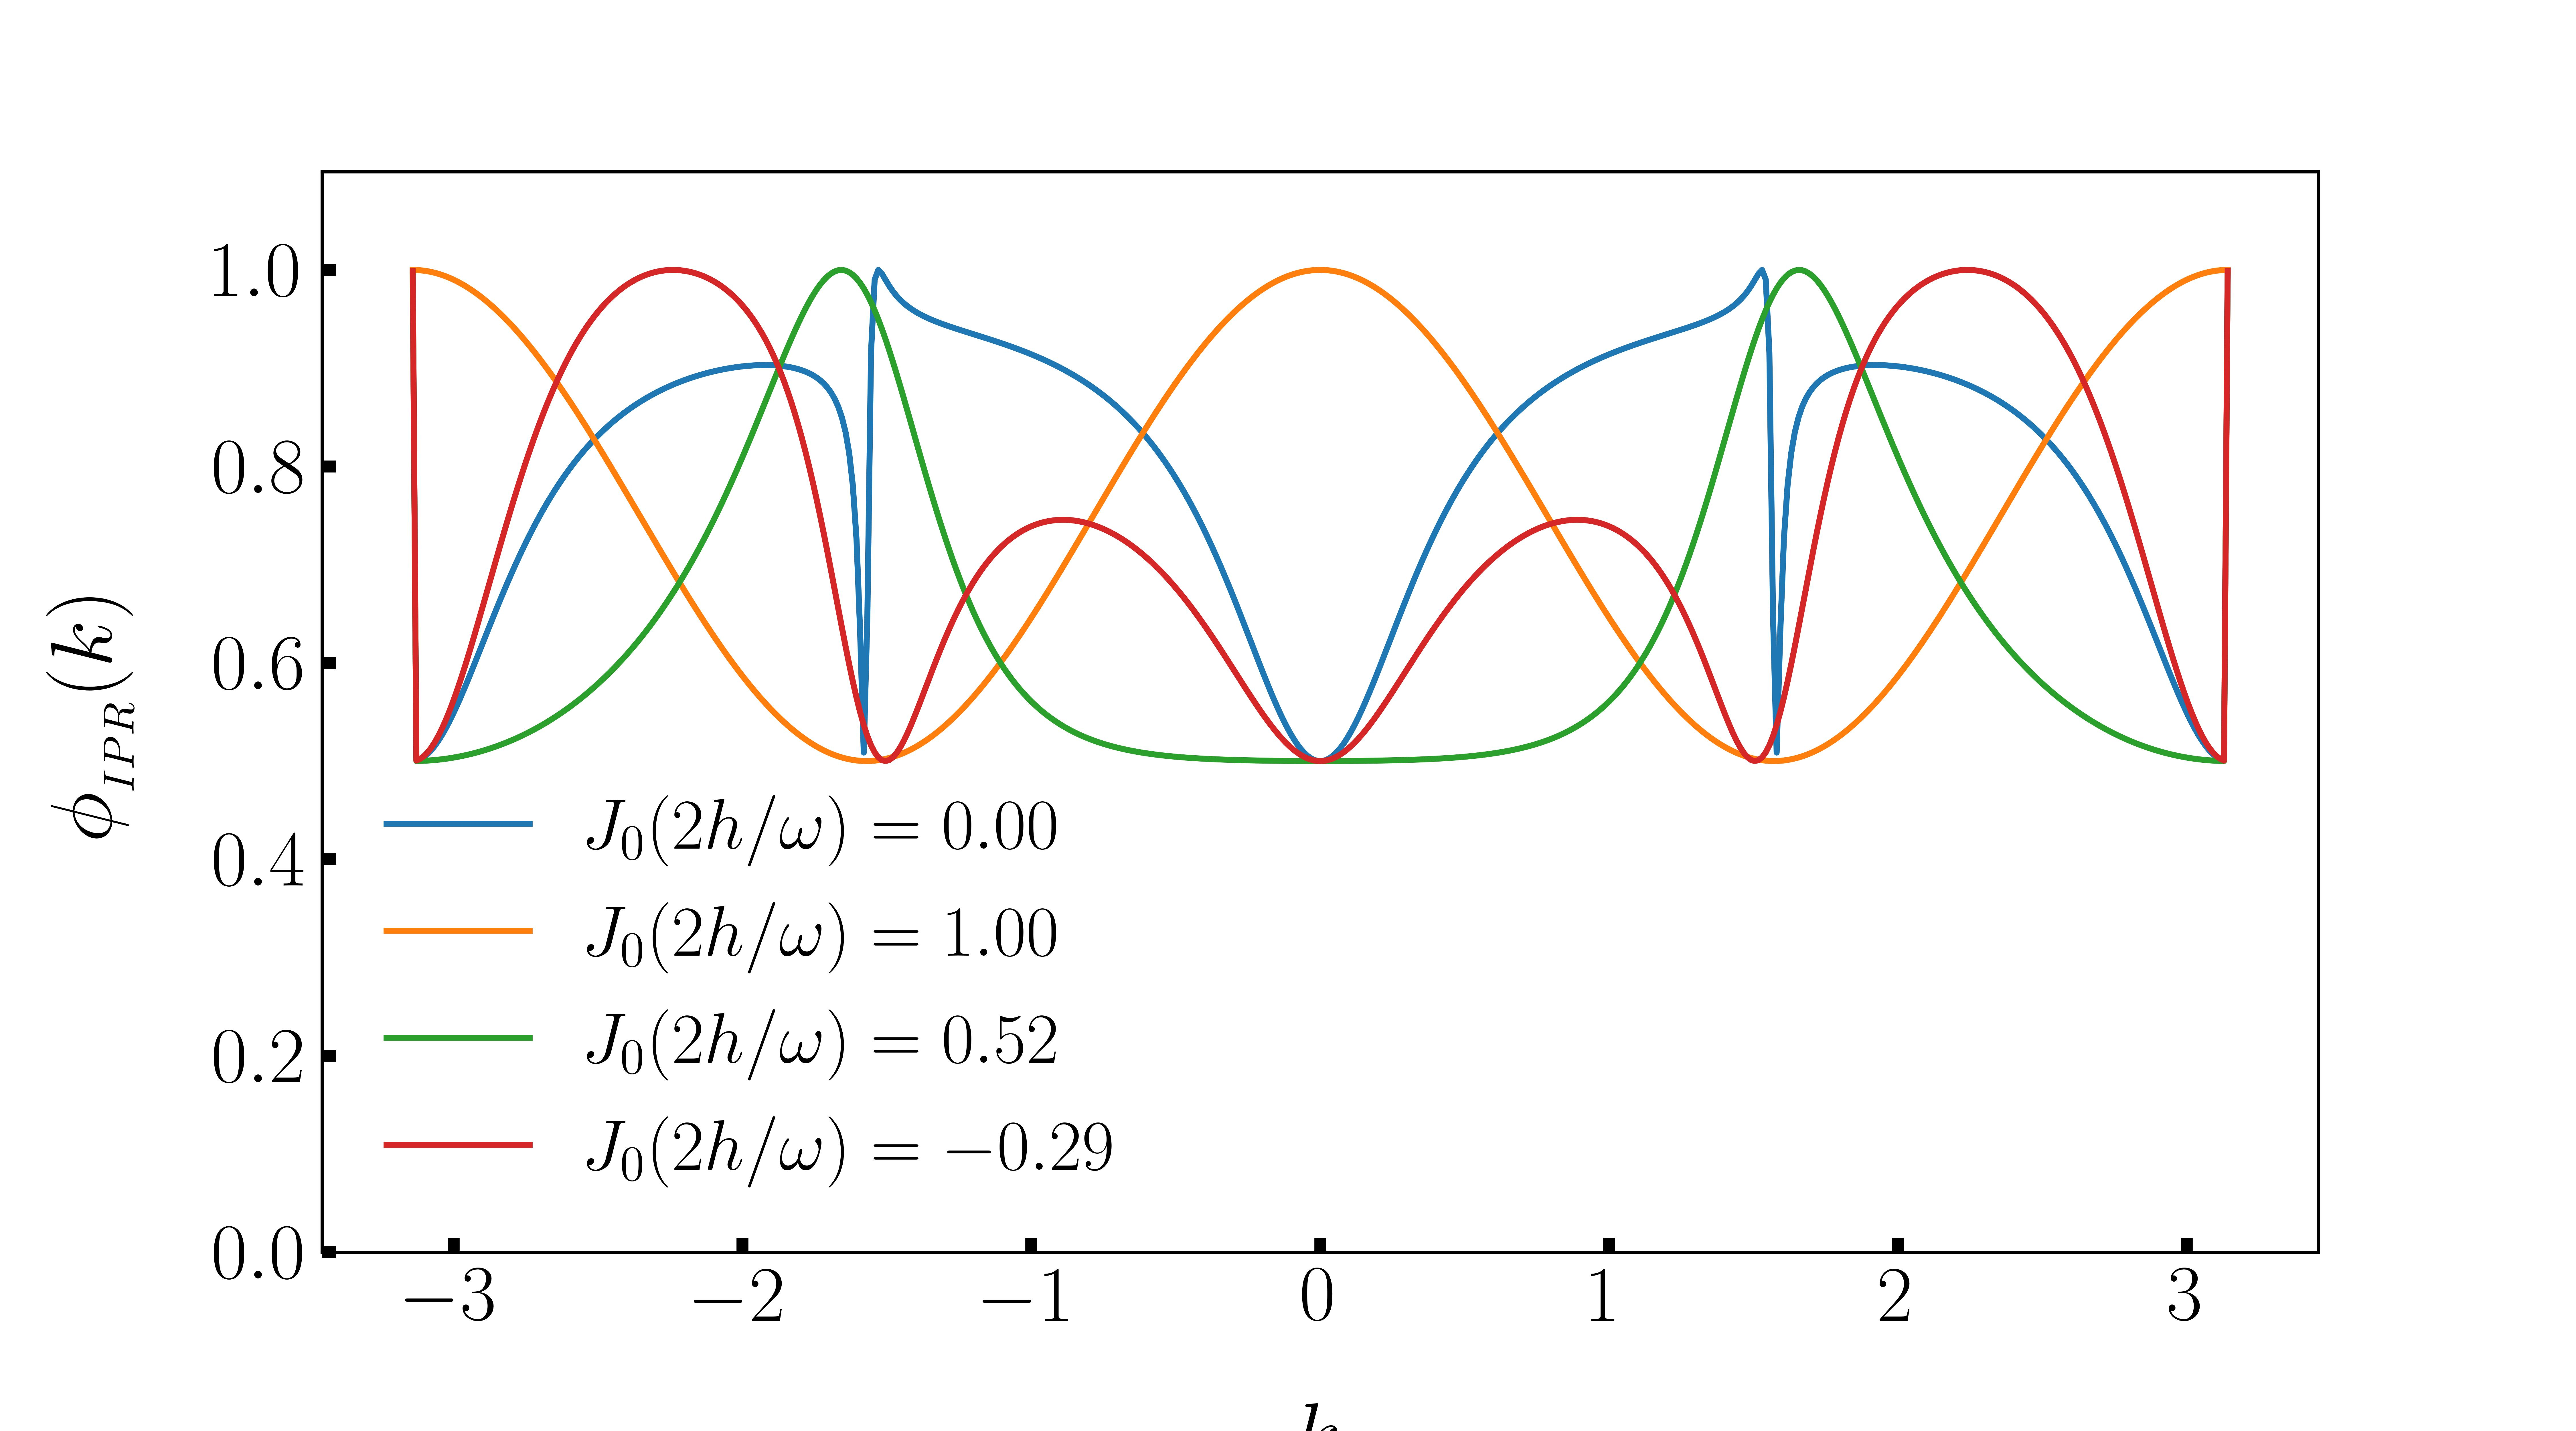
\includegraphics[height = 8.0cm, width =13cm]{low_frq_exactN500_ipr.jpeg}
\caption{\color{blue} A low frequency regime $\omega$ = 2.0 plot for IPR for Ising model at four different density points for system size N $~$ 500. IPR localization persists nonetheless. }
\end{figure}

\section{The Long-Range case: LMG model}

Consider the Hamiltonian of the type
\begin{equation}
\hat{H}(t) = \hat{H}_0 + \left(h \cos{(\omega t)} + h_0\right)\; \hat{H}_1,
\end{equation}

where

\begin{eqnarray}
\hat{H}_0 &=& \frac12 \sum_{ij}J_{ij}\hat{\sigma}^z_i\hat{\sigma}^z_j,\\
\hat{H}_1 &=& \sum_i\hat{\sigma}^x_i.
\end{eqnarray}
here,
\begin{equation*}
J_{ij} =\frac{J_\alpha}{N^{1-\alpha}}\frac{1}{r_{ij}}.
\end{equation*}
Putting  $\alpha = 0$ yields the Lipkin Meshkov Glick (LMG) \cite{lipkin64} model with all-to-all interaction, yielding $J_{ij} = J_0/N$. We choose to maintain the extensivity of the interaction energy by enforcing the condition
\begin{equation*}
\frac{J_0}{N} \sum_{i\neq j}1=\frac{J_0}{N}\frac{N(N-1)}{2}=1\\
\end{equation*}
yielding the Kac-norm $J_0=2/(N-1)$. Here, we have $N$ spin-$1/2$ particles in a $1-$dimensional lattice, and $i,j$ are site indices. We will now attempt a numerical evaluation of
the Floquet eigenspectrum of this system.

First, define permutation operator $P_{ij} = \displaystyle\frac{1}{2}\left(1+ \vec{\sigma}_i\cdot\vec{\sigma}_j\right)$,
and note that $[P_{ij}, H]=0$. Thus, we can reduce the problem size from the full $2^N\times 2^N$ Hilbert space
to the subspace spanned by the degenerate eigenvectors of $P_{ij}$ corresponding to a single eigenvalue, say $1$.
This is isomorphic to the subspace spanned by degenerate eigenstates of the operator $S^2=|\vec{S}|^2$ with eigenvalue
$\displaystyle\frac{N}{2}\left(\frac{N}{2}+1\right)$, where

\begin{equation}
\vec{S}=S^x\hat{x}+S^y\hat{y}+S^z\hat{z}\equiv\frac12 \sum_i \vec{\sigma}_i.
\end{equation}

Note that, since $[S^2, S^z]=0$, these are also eigenstates of $S^z$ in this so-called
TSS subspace. The corresponding eigenvalues are $Ns_n$, where $s_n=-\frac{1}{2}+\frac{n}{N}$ and the index
$n= 0 (1) N$ has $N+1$ values \cite{Mori}. Thus

\begin{equation}
S^z |s_n\rangle = Ns_n|s_n\rangle,
\end{equation}

and the matrix elements $(S^z)_{ij} = Ns_s\delta_{ij}$. Furthermore, defining ladder operators

\begin{equation}
S_\pm \equiv S^x \pm i S^y,
\end{equation}

and using the result

\begin{equation}
S_\pm |s_n\rangle = \sqrt{\frac{N}{2}\left(\frac{N}{2}+1\right) - Ns_n\left(Ns_{n\pm 1}\right)}\;\;|s_{n\pm 1}\rangle,
\end{equation}

we can obtain the matrix elements $S^x = S_+ + S_-$ to be

\begin{equation*}
(S^x)_{nm} = \frac{1}{2}\bigg[\sqrt{\frac{N}{2}\left(\frac{N}{2}+1\right) - Ns_n\left(Ns_{n + 1}\right)}\;\;\delta_{n+1, m}  
                        +\;\sqrt{\frac{N}{2}\left(\frac{N}{2}+1\right) - Ns_n\left(Ns_{n- 1}\right)}\;\;\delta_{n-1,m}\bigg]
\end{equation*}

Note that, considering $i<j$ the Hamiltonian can be readily written as
$H(t) = -\displaystyle\frac{2}{N-1}(S^z)^2 - 2(h \cos{(\omega t )} + h_0)S^x$, the matrix elements of
\begin{align*}
\left(H_0\right)_{ij} &= -\frac{4}{N-1} s^2_i \delta_{ij},\nonumber\\
\left(H_1\right)_{ij} &= \bigg[\sqrt{\frac{N}{2}\left(\frac{N}{2}+1\right) - Ns_i\left(Ns_{i + 1}\right)}\;\;\delta_{i+1, j}  
                        +\;\sqrt{\frac{N}{2}\left(\frac{N}{2}+1\right) - Ns_i\left(Ns_{i- 1}\right)}\;\;\delta_{i-1,j}\bigg]
\end{align*}

Note that, in the continuum limit, $N\rightarrow\infty$, we can ignore the difference between adjacent values
of $s_i$. Thus, the Hamiltonian per particle becomes $h(t)\equiv \displaystyle\frac{1}{N}H(t) = h + h_0\cos{(\omega t)}h_1$, where

\begin{eqnarray}
\left(h\right)_{ij} &\approx& - 2s^2_i \delta_{ij},\nonumber\\
H_0 &\rightarrow& -2s^2\\
\left(h_1\right)_{ij} &\approx& \sqrt{1 - 4s^2_i}\left[\delta_{i+1, j}  + \delta_{i-1,j}\right]\\
H_1 &\rightarrow& \sqrt{1 - 4s^2_i}\;\;\cos{p},
\end{eqnarray}
where we have expanded the matrix elements in a basis of $e^{ipx}$.


This Hamiltonian can be simplified in the Rotated Basis as follows. Transform the Hamiltonian to the frame given by the transformation \cite{ArnabD}

\begin{equation*}
\hat{U}(t)=\exp \left[i \frac{h}{\omega} \sin (\omega t) \hat{H}_{1}\right]
\end{equation*}
Defining $\tau = \displaystyle\frac{h}{\omega}\sin{\omega t}$, we use the fact that $\hat{H}_1 = 2 S^x$, and the identity  $e^{i 2\tau\hat{S^{x}}} \hat{S^{z}} e^{-i 2\tau \hat{S^{x}}}=\hat{S^{z}} \cos \left(2\tau\right)+\hat{S}^{y} \sin \left(2\tau\right)$ to simplify the transformed Hamiltonian, yielding
\begin{equation*}
\tilde{H}(t)= -\frac{1}{N-1}\Bigg[\big(S^z\big)^2 \big(1+\cos{4\tau}\big) + \big(S^y\big)^2 \big(1-\cos{4\tau}\big) + \big\{S^y, S^z\big\}\sin{4\tau}\Bigg] - 2 h_0 S^x
\end{equation*}

Now, we know that $\hat{S}^{2}=\big(\hat{S}^x\big)^{2}+\big(\hat{S}^y\big)^{2}+\big(\hat{S}^z\big)^{2}=\frac{N}{2}\left(\frac{N}{2}+1\right)$ when the system is confined to the TSS subspace. In addition, we define $\eta\equiv 4h/\omega$ and use the Jacobi-Anger formulae

\begin{align*}
\cos \big(\eta \sin\omega t\big) &= J_{0}(\eta)+2 \sum_{n=1}^{\infty} J_{2 n}(\eta) \cos (2 n \omega t) \\
\sin \big(\eta \sin\omega t\big) &= 2 \sum_{n=1}^{\infty} J_{2 n-1}(\eta)\sin [(2 n-1) \omega t]
\end{align*}
to simplify the expression for $\tilde{H}(t)$. Finally, we assume that the drive frequency $\omega$ is large enough that all harmonic terms in the Hamiltonian can be averaged out over discernible time scales. This yields the Hamiltonian in the Rotated Wave Approximation (RWA) to be (ignoring constant terms in the addition)

\begin{equation*}
\tilde{H}_{\mathrm{RWA}}= \frac{\big(\hat{S}^x\big)^{2}}{N-1} - 2h_0 \hat{S}^x - \frac{J_0(\eta)}{N-1}\bigg[\big(\hat{S}^z\big)^{2} - \big(\hat{S}^y\big)^{2} \bigg]
\end{equation*}


Now, if the drive amplitude $h$ is adjusted such that $\eta$ lies at a root of $J_0(\eta)$ (the localization point), the RWA Hamiltonian is diagonal in the representation of the transverse field $\hat{S}^x$, yielding an IPR of unity in that representation, similar to the Ising case. Note however, that if the DC transverse field $h_0$ is set to $0$, then, at the localization point, the RWA Hamiltonian $\tilde{H}_{\mathrm{RWA}}\sim
\big(\hat{S}^x\big)^2$, each of whose eigenvalues (given by $\big(\frac{N}{2}-m\big)^2$ where $m \in 0(1)N$, and $\big(\frac{N}{2}-m\big)$  are the eigenvalues of $\hat{S}^x$) are **two-fold degenerate. This produces infinitely many (Floquet) eigenmodes in the degenerate subspace whose IPRs may not always be unity** in the $S^x$ representation. Thus, the absence of the DC field may produce delocalization in the Floquet states even at the localization points, and this necessitated the inclusion of a DC field $h_0$ in order to break the symmetry.
Finally, note that not all values of the DC field $h_0$ removes all degeneracies in $\tilde{H}_{\mathrm{RWA}}$. To see this, note that, at the localization point, the eigenvalues of $\tilde{H}_{\mathrm{RWA}}$ are given by

\begin{equation*}
\rm{Eigs}\bigg[\tilde{H}_{\mathrm{RWA}}\bigg] = \frac{\bigg(\frac{N}{2}-m\bigg)^2}{N-1} - 2h_0 \bigg(\frac{N}{2}-m\bigg).
\end{equation*}

In order to ensure that no degeneracies occur, we have to adjust $h_0$ to ensure that for any two integers $m_1, m_2 \leq N$  the condition below is always met


\begin{equation*}
\frac{\bigg(\frac{N}{2}-m_1\bigg)^2}{N-1} - 2h_0 \bigg(\frac{N}{2}-m_1\bigg) \neq \frac{\bigg(\frac{N}{2}-m_2\bigg)^2}{N-1} - 2h_0 \bigg(\frac{N}{2}-m_2\bigg).
\end{equation*}

If $N\gg 1$ (substantially large), then this condition can be met by assuring that $(1-2h_0)^{-1}$ is never an integer that is divisible by $N$. To ensure this in our simulations below, we keep $h_0$ at an **irrational** value of $\sqrt{3}$.


This result is tentatively supported by exact simulations, as can be seen in the plots below. There, we show plots of the IPR of the Floquet mode $|\phi^n\rangle$ for all $n$ corresponding to eigenvalues of $S^x$ for a fixed eigenvalue of $S^2 = N/2\big(N/2 + 1\big)$. The IPR is thus
\begin{equation*}
\phi_{IPR}(n) = \sum_m \left\vert\langle m\vert\phi^n\rangle\right\vert^4,
\end{equation*}
where $|m\rangle$ is the $m^{th}$ eigenstate of $\hat{S}^x$


Now, we look at numerical simulations for $H(t)$ via the IPR of the Floquet state in the representation of the transverse field *i.e.* the eigenstates of $S^x$. We're keeping $\omega = 90$ as a large enough value for RWA to hold, and $N=\mathcal{O}(10^2)$ which our computational resources will allow. 

\begin{figure}[ht!]
\centering
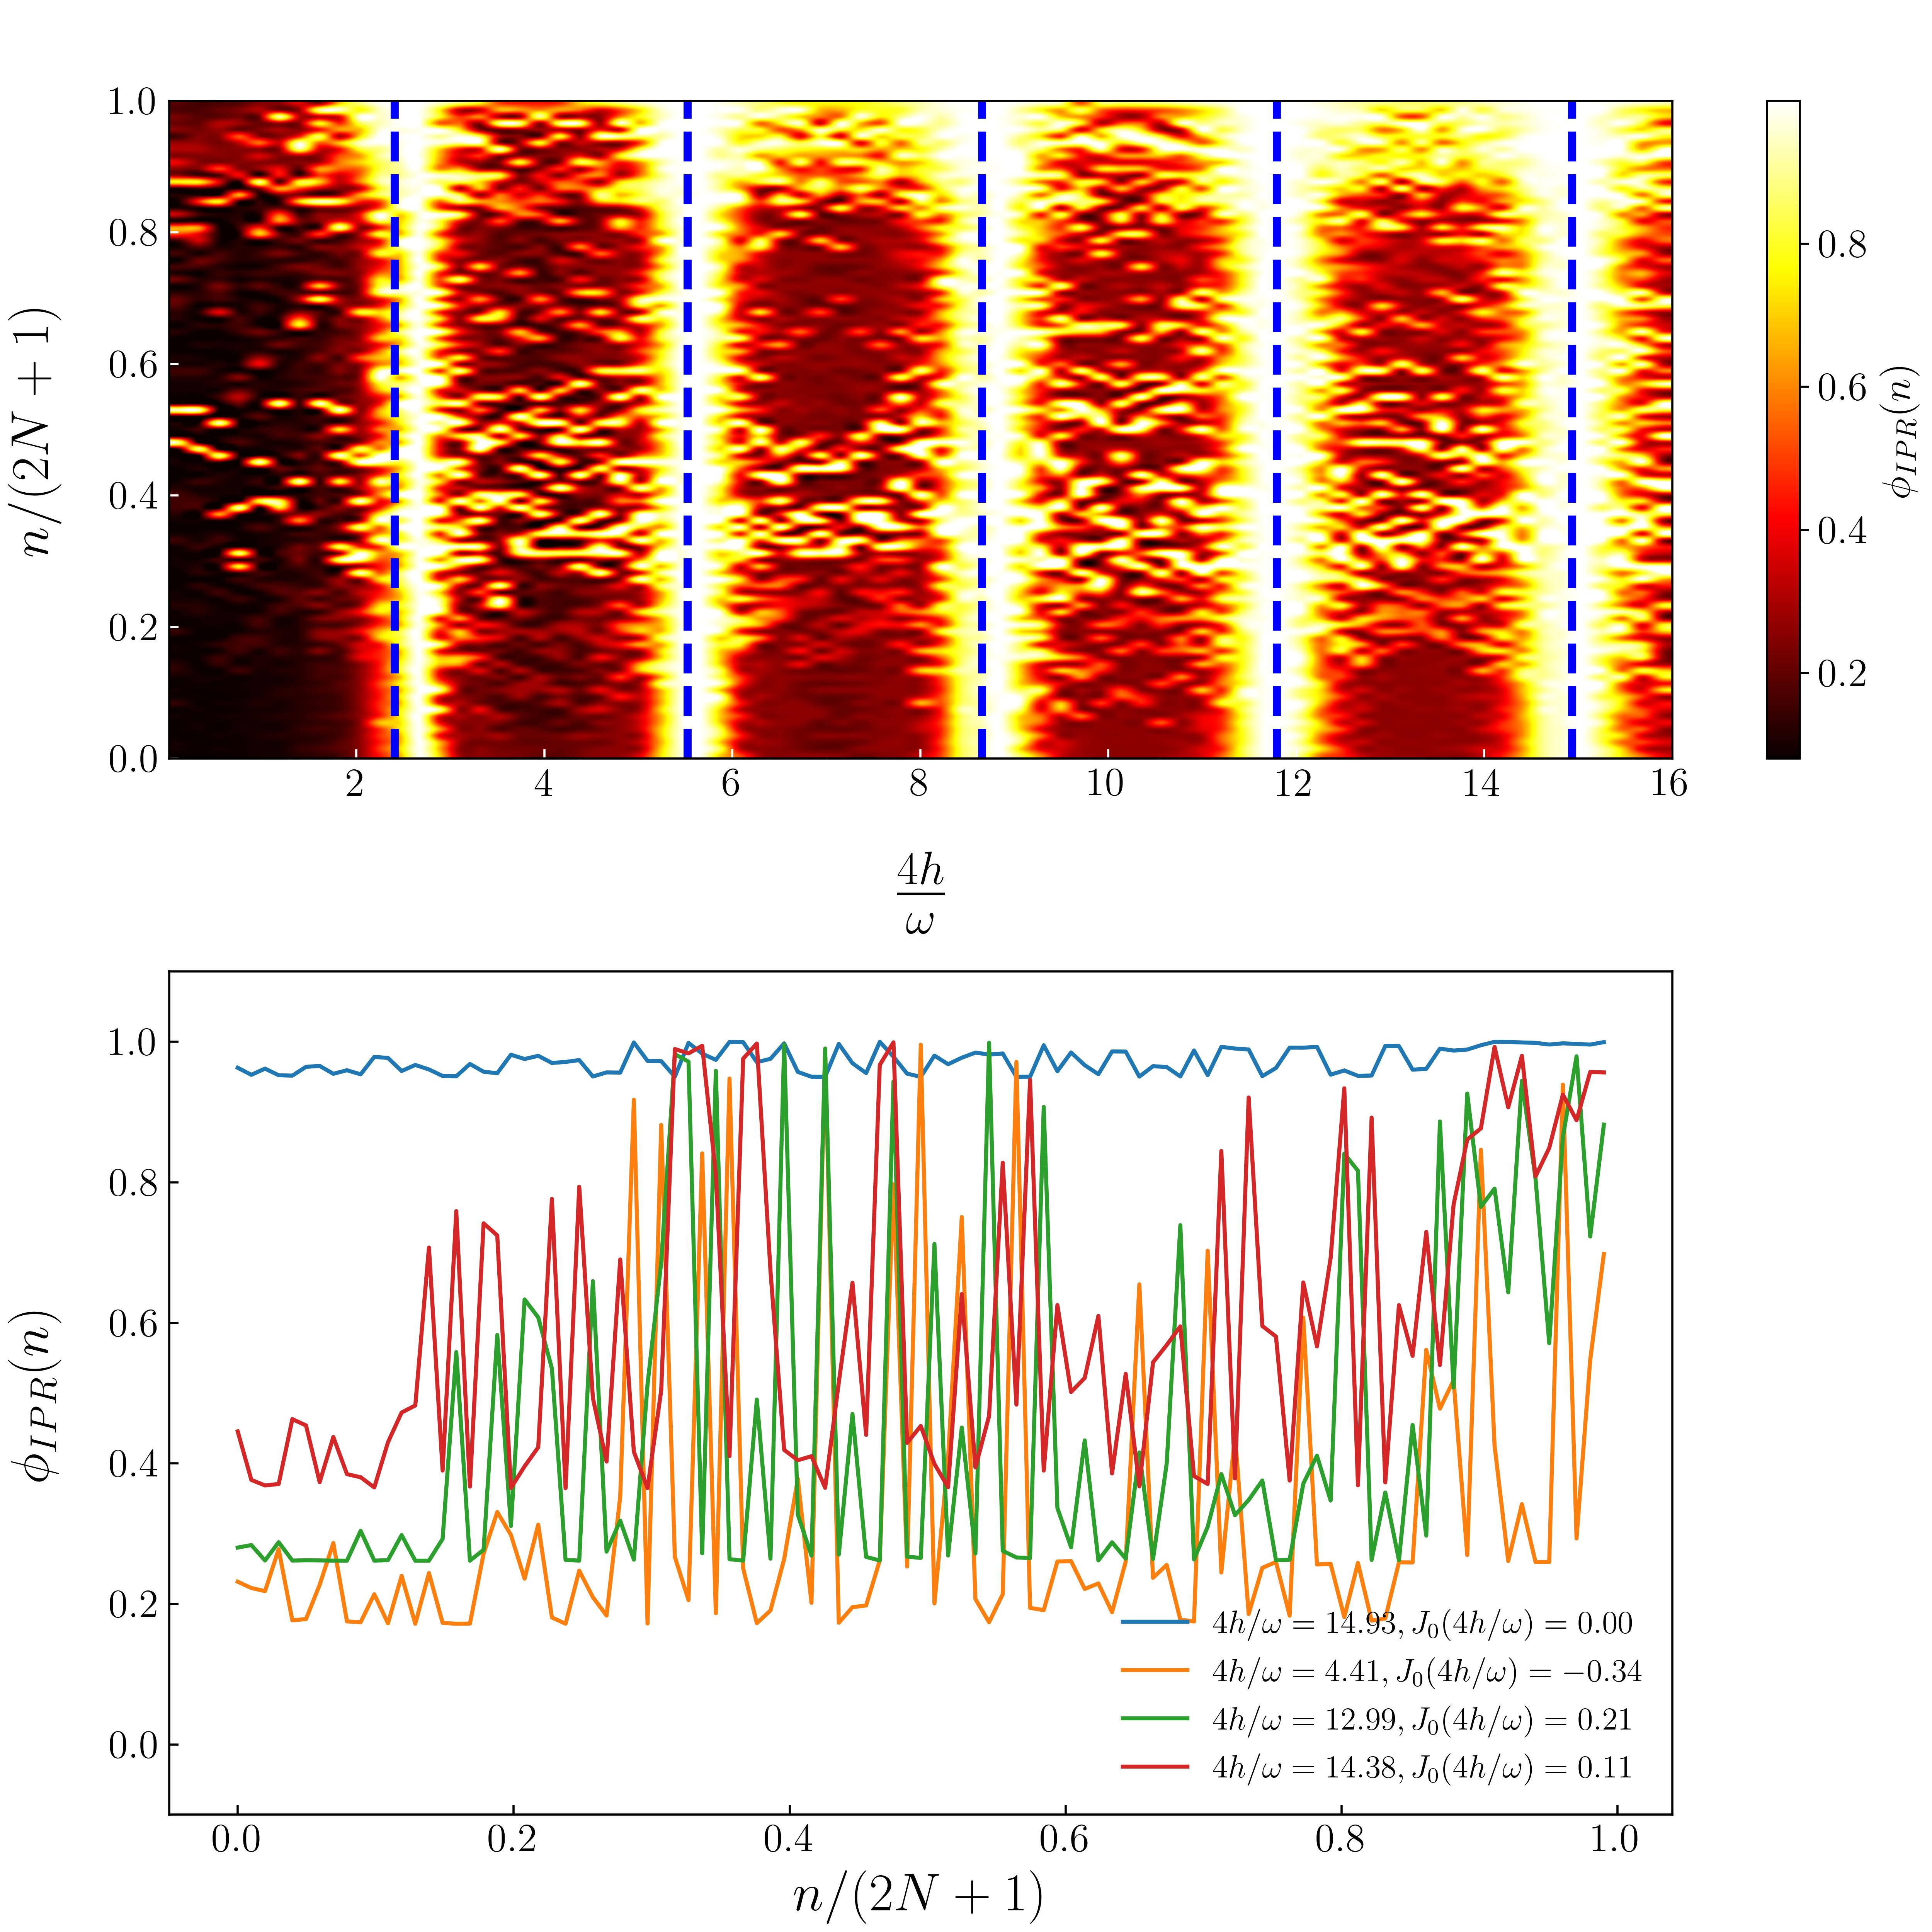
\includegraphics[height = 12.0cm, width =12cm]{ipr_exact_dynm_N50_frq_90_.jpeg}
\caption{\color{blue}The IPR for exact dynamics for spin model size N$\sim$ 30. The upper panel shows density plot of IPR of Floquet modes for different parameter points corresponding to ratio between strength and the frequency of the symmetry breaking field which is the lowest root among Bessels roots of first kind and zeroth order $\frac{4h}{\omega}$. The dc part of the symmetry braking field is kept at a small irrational number to avoid the symmetry arising from degeneracy in flqouet states. The IPR density is high at Bessels first order roots, $J_0\Big(\frac{4h}{\omega}\Big)=0$ for all the available floquet states. The lower panel shows the crossectional plot of IPR for four different floquet IPR density points. The point corresponding $J_0\Big(\frac{4h}{\omega}\Big)=0$ has ~unity value for all states where at points away from the roots have lower and high fluctuations.}
\end{figure}
The top panel has a density plot of the IPR of the Floquet states, with $\eta=4h/\omega$ on the abscissa and the spin index $m/(2N+1)$ on the ordinate. The dashed vertical lines correspond to roots of $J_0(\eta)$. As can be seen, the IPR is essentially unity at large roots of $J_0(\eta)$, indicating complete Many Body localization. However, there is some departure from unity at the smallest root of $J_0(\eta)$. This is due to the fact that at the smallest root of $J_0(\eta)\approx 2.405$, the amplitudes of the contributions of the higher order terms in the RW expansion, which are of $\mathcal{O}(J_n(\eta))$, are large enough to contribute to delocalization.

The bottom panel contains cross sections of the full IPR plot for select values of $\eta$ as indicated in the legend. Here, we can see more clearly that, when the drive amplitude $h$ is adjusted to make $J_0(\eta)\neq 0$, the Floquet States are mixed, but not entirely thermal, since the IPR does not fall to $\mathcal{O}(N^{-1})$, indicating that localization persists to some extent always.

\indent So, as long as there is an appropriate DC field, $S^x$ is mostly conserved and $H_F$ is mostly diagonal in the $S^x$ representation at freezing point. The small deviations from this conservation occur due to the role of higher order terms in the Fourier expansion of the Hamiltonian on the rotating basis that contribute additional time-periodic terms to the RWA Hamiltonian, as can be seen below.


\section{RWA to higher orders}

The full Hamiltonian for the LMG model in the rotated basis is

\begin{multline*}
\tilde{H}(t)\sim \frac{\big(\hat{S}^x\big)^{2}}{N-1} - 2h_0 \hat{S}^x - \frac{J_0(\eta)}{N-1}\bigg[\big(\hat{S}^z\big)^{2} - \big(\hat{S}^y\big)^{2} \bigg] - \frac{2}{N-1}\sum^\infty_{n=1}\;J_{2n}(\eta)\;\Big[\big( \hat{S}^z\big)^2 - \big( \hat{S}^y\big)^2\Big]\;\cos{\big(2n\omega t\big)}\\
- \frac{2}{N-1}\sum^\infty_{n=1}J_{2n-1}(\eta)\;\big\{ \hat{S}^y,  \hat{S}^z \big\}  \;\sin{\Big[\big(2n-1\big)\omega t\Big]}
\end{multline*}
\begin{figure}[ht!]
\centering
\includegraphics[height = 9.0cm, width =10.0cm]{comprasion_LMG_50_highFr90_exact_nd_rwa.jpeg}
\caption{\color{blue}The comparison between IPR for exact dynamics and RWA with corresponding correction orders shows that IPR variation for exact dynamics for LMG model approximately can be described by the RWA with higher correction orders.}
\end{figure}


\section{ Classical Lipkin Dynamics}

In the continuum limit, the Lipkin system can be described by the $p,q$ Hamiltonian:
\begin{equation*}
H = -2 q^2 - h(t)\;\sqrt{1-4q^2}\;\cos{p},
\end{equation*}
which yields the Hamiltonian dynamical system 
\begin{align*}
\frac{dq}{dt} &= h(t)\;\sqrt{1-4q^2}\;\sin{p}\\
\frac{dp}{dt} &= 4q\bigg[1-\frac{h(t)\cos{p}}{\sqrt{1-4q^2}}\bigg]
\end{align*}
Below are the Poincare sections (strobed at integer multiples of $T=2\pi/\omega$) of the ensuing dynamics for $h(t)=h\cos{\omega t}$ for two cases, one for which $J_0(4h/\omega)=0$ and one at a lower value of $h$. These are compared with the Husimi Q-functions of the Floquet States obtained above. The quantum phase space is described by the Spectral Average of the Husimi functions of all the Floquet modes $|\phi^n\rangle$ for the chosen value of $S^2$, i.e. for a coherent state $|q, p\rangle$, we plot
\begin{equation*}
H(q,p)\equiv \frac{1}{\big(2N+1\big)\pi}\sum_n \langle q,p\vert \phi^n\rangle\langle\phi^n\vert q,p\rangle
\end{equation*}

These are shown for two cases, small $\omega$, where the classical plots are chaos dominated, and large $\omega$, where they are regular.
\begin{figure}[ht!]
\centering
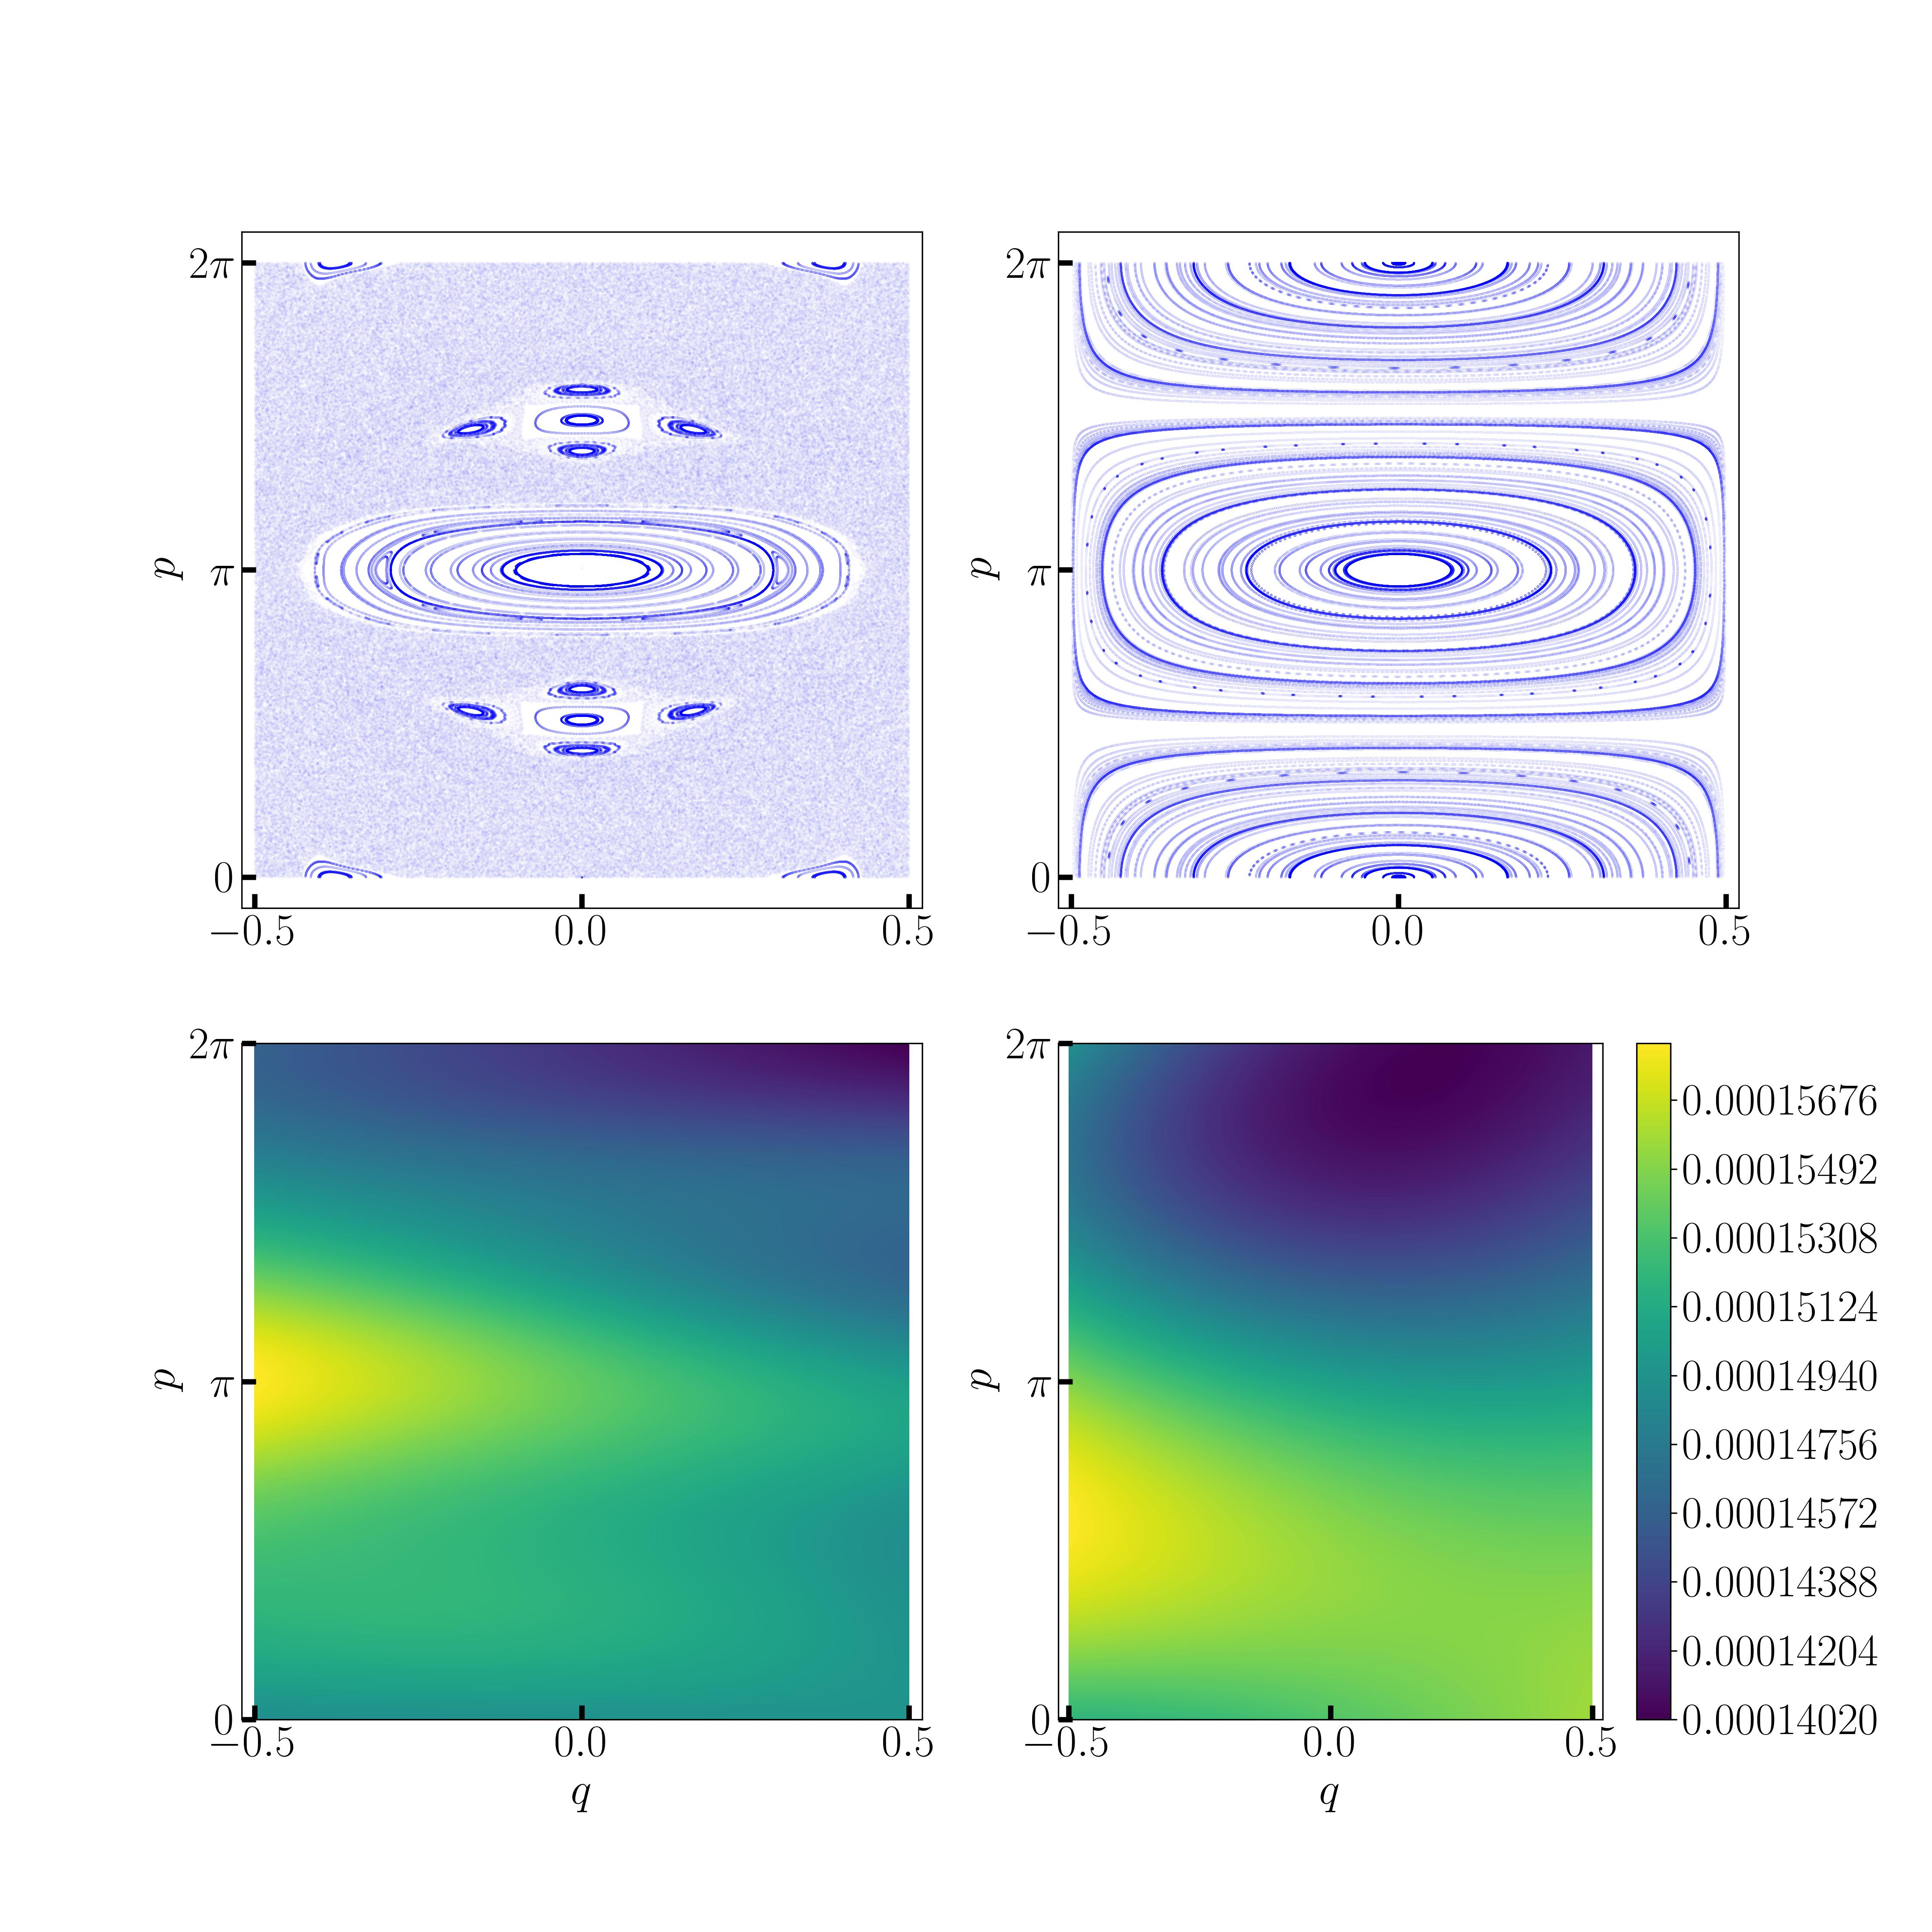
\includegraphics[height = 12.0cm, width = 12cm]{lmg_poincare.jpeg}
\caption{\color{blue}The above panel describes the phase-space Poincare distribution symmetry breaking smaller drive frequency (left) and higher frequency (right) for system size N = 500 with 100 realisation numbers. At smaller frequencies the Poincare picture contains chaotic behavior (top left panel) where at the higher frequencies it is a normal Poincare picture which represents discrete freezing behaviour(top right panel). The bottom panel is Hushimi Q-function average plot for  smaller frequency (bottom left) has a uniform distribution with less contrast in color. This means a Q-function distribution in chaotic behavior. At the right bottom the Hushimi plot has distinct contrast in Q-function average value which represents a regular dynamics pattern in system.}
\end{figure}

At low drive frequencies, the onset of chaos in the thermodynamic limit suggests that the IPR of the Floquet states should be delocalized. This is shown in the output of the code cell below.

\section{Thermality to Athermality: A Phase Transition}

We contrast the Floquet-IPR behaviour of both the periodically driven Ising model and the periodically driven LMG model. 

\begin{figure}[!ht]
\centering
\includegraphics[width = 10.0cm, height =10.0cm]{phase_transition_LMG_N.jpeg}
\caption{\color{blue} For different spin sizes IPR plotted at  Bessel's first root with first kind $J_0\Big(\frac{4h}{\omega}\Big)$ varying both the drive amplitude and frequency in LMG spin array. The drive frequency is increased adiabtically from sufficiently low frequency O(1) and  up-to high frequency O(50) for system size N = 10,20,30,50,100. IPR found to be low enough at small frequency up to a critical frequency where IPR rises to unity abruptly for each system sizes(Top panel) .  It is also found that at low frequency region the system IPR decreases in scale of N which confirms distribution of participation of the states of the system (Bottom panel). The change in IPR at critical frequency is sharper as system size increases more, this indicates at infinite large system ($N\xrightarrow{}\infty$)the the change in IPR to unity is instantaneous resulting  a phase transition at critical frequency.}
\end{figure}


\begin{itemize}

\item For the Ising model at large $h, \omega$, we can see clear localization at freezing points, obtained by fixing $J_0(2h/\omega)=0$,  for both the exact and Rotated Wave simulations, with fairly weak delocalization away from these freezing points. 

\item Since the Ising model is integrable, we can see localization even at small values of $\omega$ despite the fact that RWA breaks down and analytical treatments beyond the adiabatic limit are complicated.

\item In the LMG model, we can see clear localization at localization points, obtained by fixing $J_0(4h/\omega)=0$, for both the exact and Rotated Wave simulations, with fairly weak delocalization away from those points.

\item However, since the LMG model is non-integrable, and the onset of chaos in the thermodynamic limit for small $\omega$ is well-known, we can observe near complete delocalization in the IPR of the Floquet states at small $\omega$.
\end{itemize}

Hence, we adiabatically vary $\omega, h$ in the LMG model, subject to the constraint that $\eta=4h/\omega$ is kept at a root of $J_0(\eta)$, there we found a crossover or phase transition from almost totally thermal to totally localized behaviour (fig 8). Even if we relax the constraint, there is a macroscopic change in behaviour from thermal to athermal. At low frequency regime IPR founds to be decreasing with scaling in system size N and when N is large i.e. $\rightarrow{}\infty$ IPR appears to vanish, thereby fully thermalized state at $\eta=4h/\omega$.  This contrasts with the Ising model, where no such transition appears. Thus, the inclusion of long-range interactions seems to induce a transition from thermal to localized phase, a feature that will prove useful in designing MBL engines.

\section{Conclusion and Outlook}

Points to enter
\begin{itemize}
	\item We have investigated the following
	\begin{enumerate}
		\item The onset of Dynamical Many Body Localization in periodically driven long-range spins.
		\item  using LMG as the paradigmatic example.
		\item Localization parametrized by the Inverse participation ratio of Floquet eigenstates.
		\item Numerically contrasted IPR of the LMG model with that of the TFIM for low and high drive frequencies.
		\item Phase space dynamics of the LMG model to investigate the onset of thermal behavior at low frequencies and localization at high frequencies. 
		\item Analytically investigate the onset of additional approximately conserved quantities in the high-frequency regime for both models.
	\end{enumerate}
\item Our conclusions:
\begin{enumerate}
	\item Long-range spins show strong localization in spin co-ordinate space for the LMG model when drive frequency $\omega \gg J$, where $J$ is the spin exchange energy. The localization occurs at specific resonances of the drive frequency and amplitude $h$, \textit{i.e.} when  $J_0(4h/\omega)=0$ for the LMG. 
	\item While similar localization (in momentum space) has been observed for the TFIM case at resonances given by $J_0(2h/\omega)=0$, the mechanism is different in long range systems due to the fact that a different observable ($(S^x)^2$ where $\mathbf{S}$ is the total spin) is approximately conserved in the LMG case.
	\item Once the accidental degeneracy is removed by a DC transverse field that goes as $\sim S^x$, the eigenstates can be mapped to a co-ordinate representation, leading to strong spatial localization.
	\item In addition, we have observed a strong mobility edge in the periodically driven LMG model as the frequency is adiabatically increased from $\omega \sim J$ to $\omega \gg J$. In the former regime, the onset of  dynamical chaos in the classical dynamics ensures that the quantum system eventually thermalizes at infinite temperature. However, this is indefinitely delayed in the latter regime due to dynamical localization.
	\item 
	The mobility edge between these regimes shows singular behavior in the thermodynamic limit, suggesting a quantum phase transition between them. This is not present in the short-range TFIM, where the IPR is too large in the low-frequency limit to induce thermal behavior.
	\item Thus, Floquet engineering in long-range systems is sufficient to induce Thermal and MBL states, and disorder is not required. 
\end{enumerate}

\item Outlook:
\begin{enumerate}
	\item We have looked at clean systems with high symmetry. The addition of integrability-breaking terms (such as disorder) should induce thermalization in all cases, but, analogous to the TFIM case (cite literature), thermalization in LMG should be delayed significantly when $\omega \gg J$ and $J_0(4h/\omega)=0$.
	\item Numerical investigations in intermediate-range spins (write Hamiltonian - $0< \beta < \infty$) using approximate methods 
	\item The phase transition allows the operation of an MBL engine in the LMG case, with a Thermodynamic cycle operating between the thermal and MBL regimes. Investigate diabatic corrections.
\end{enumerate}
\end{itemize}



\printbibliography %Prints bibliography
\end{document}